\section{Lois, you were the 9th generation of Hess's born in the land in Lancaster County.
Can you talk about your family's relationship with the land over time and what that looked like? How did your family's longevity on the land impact relationships at church and elsewhere?}
There is an interesting difference between my paternal grandparents and their relationship to the land.
Christian my Grandfather Hess died when my father was less than two years old.
I never knew much about him except for his dying story.
Which I may have told you in another place.
If not I can add it here.
Below I'll talk more about the Hess connection to land.
As a widow his wife, Mary, the only grandparent I knew, bought one of the three farms my Grandfather Emanuel Groff owned.
This made it possible for my father to begin buying a farm as a young man.

\begin{figure}
\centering
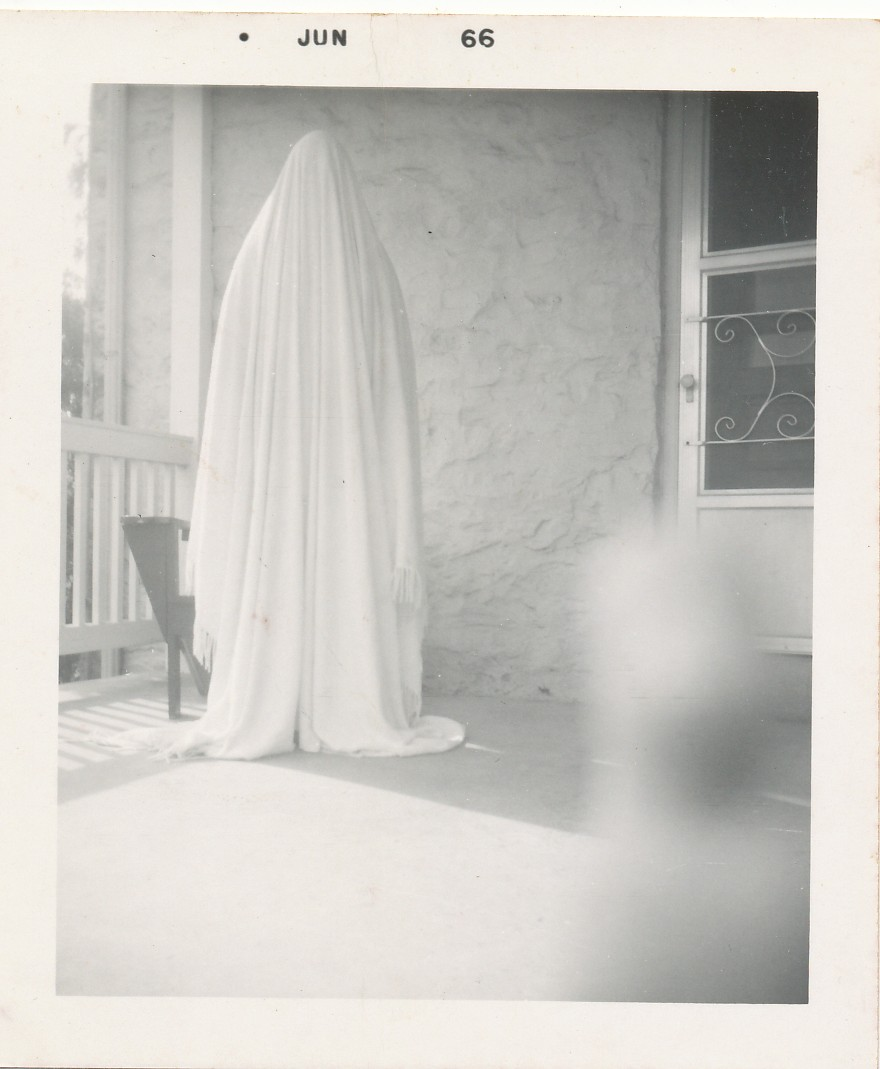
\includegraphics[width=0.9\textwidth]{reflections/1.jpg}
\caption{
Looking down the lane to the farm on Second Lock Road
}
\end{figure}

Interestingly I do not know much about my Hess great grandparents, Benjamin H.
and Emma Hess.
My mother writes on page 80 of the book The Fruitful Vine, that neither she nor my father knew much about them.
Since my father also did not know his father there is a two generation gap of information.

My mother writes of a visit she and Pop made to an Uncle Henry R Hess in May 1968 to learn more about Benjamin H Hess.
Here is some of what she wrote.

      "He was a big man over 6 feet tall.
He had big hands and was able to accomplish a lot of work in a short time.
They owned and farmed a farm near Marticville, PA.
He loved to sing, and in the evenings he would often take a hymn book and sing by himself, if no one else was inclined to sing with him.
If anyone in the neighborhood was sick or in trouble he was quick to offer help.
He often stayed up at night with people who were sick."
"
Marticville is in southern Lancaster County.
While Lancaster County is known for fertile farm land the southern part had rolling hills with rocks and the land was not as fertile.
The farmers there were not as successful.

The description of Benjamin Hess could also be a description of my father.
He was 6 feet tall, had big hands and worked hard.
I remember noticing that the blue denim shirts he wore for farm work were often wet with sweat when he came in from working.
He too enjoyed singing but during a softball game was hit on the throat by a ball.
The injury affected his singing voice.
He too was willing to help others in trouble.
He enjoyed serving with MDS (Mennonite Disaster Service) at various times.
He wanted to be a good farmer and was one of the first farmers in the area to contour the fields of his farm to prevent runoff after heavy rains and snows.

\begin{figure}
\centering
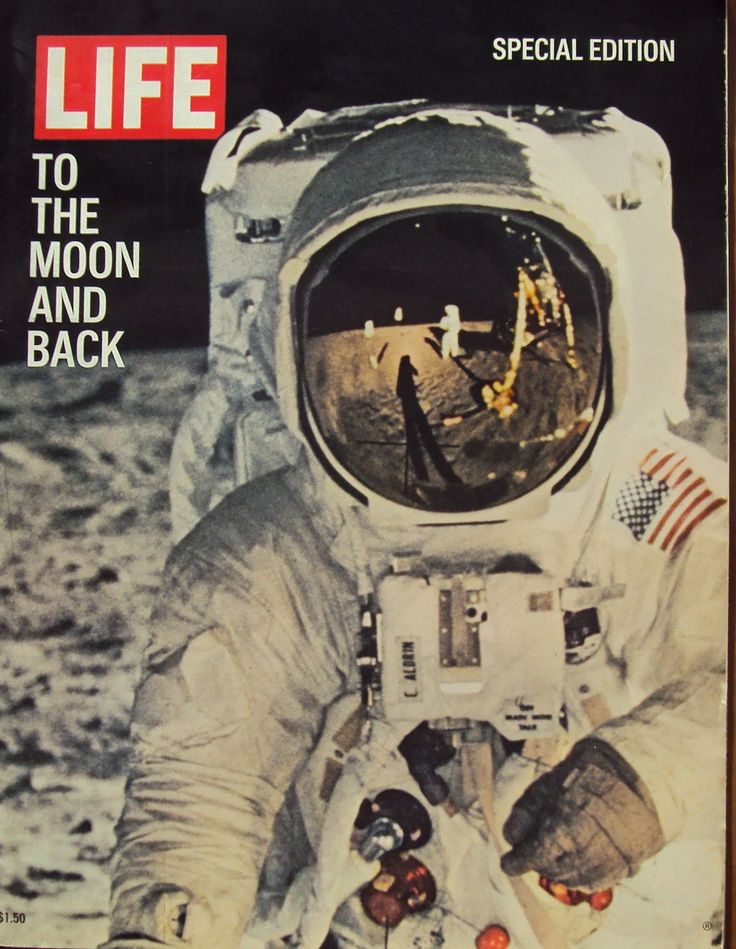
\includegraphics[width=0.9\textwidth]{reflections/2.jpg}
\caption{
Young farmers, Mary and Jacob Hess
}
\end{figure}

Mary, the widow of Christian Hess, was the only grandparent that I knew.
She was a quiet presence in my life and I feel that I only knew her in a somewhat superficial way.
There are stories about her parents, my great-grandparents Emanuel and Susie Groff.
Emanuel owned three farms by the time my grandfather Christian was ready to marry Mary and begin farming one of the Groff farms.

\begin{figure}
\centering
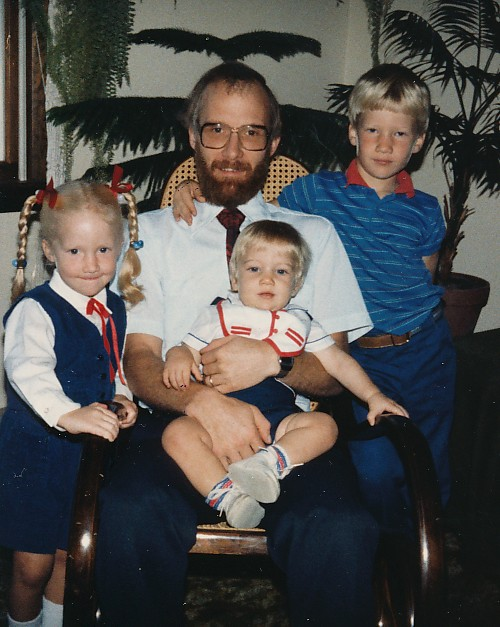
\includegraphics[width=0.9\textwidth]{reflections/3.jpg}
\caption{
Christian and Mary Hess
}
\end{figure}
After Christian died Mary moved home to her parent's house.
Her children lived there while she went from family to family caring for the family when a baby was born.
Some of my older brothers and sisters remember visiting Emanuel and Susie.

\begin{figure}
\centering
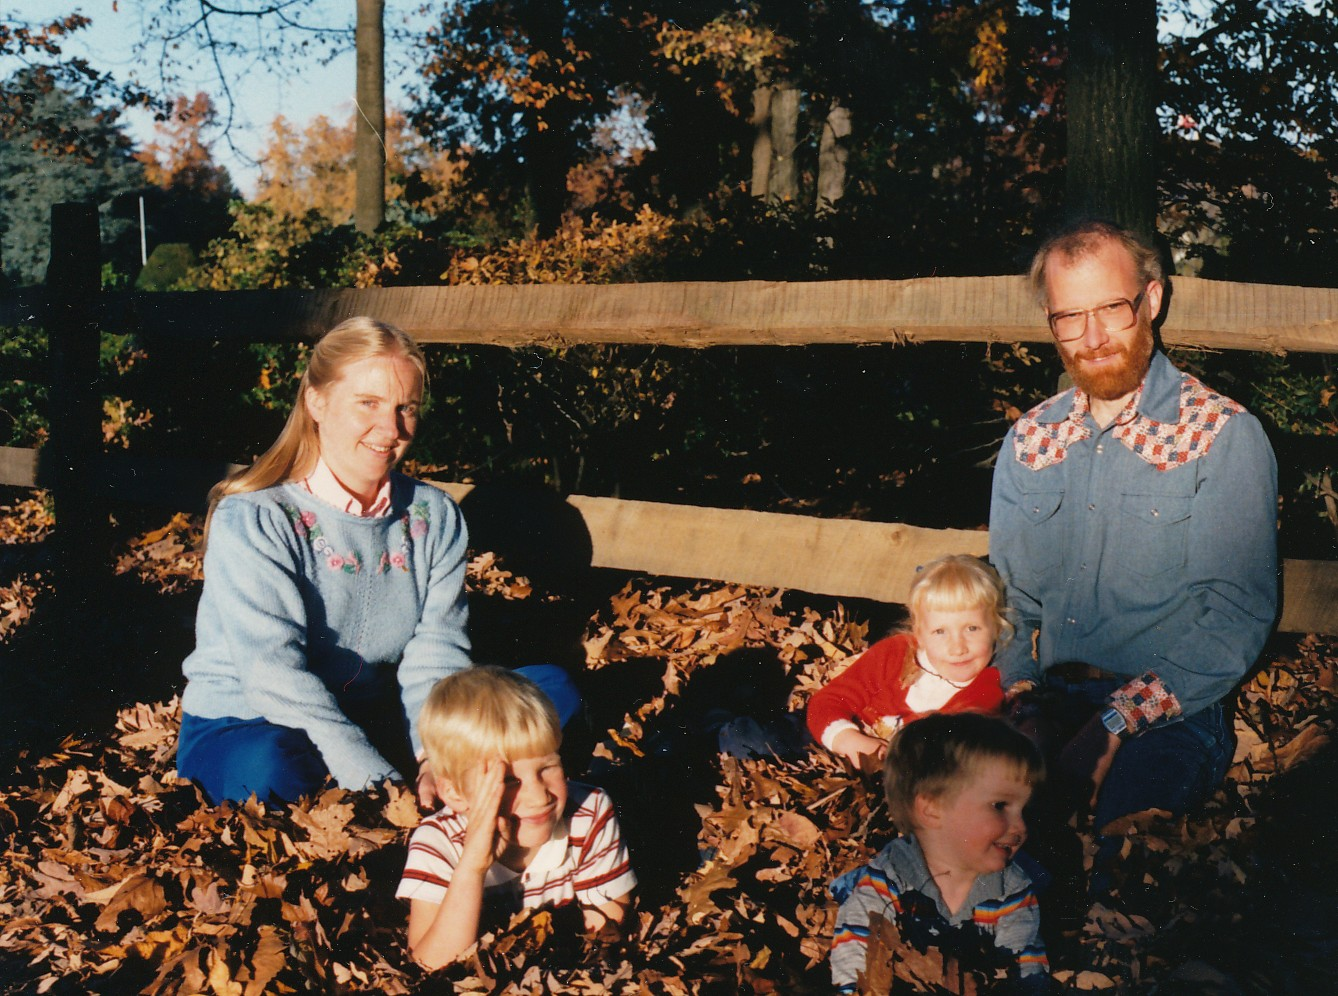
\includegraphics[width=0.9\textwidth]{reflections/4.jpg}
\caption{
Susie and Emanuel Groff
}
\end{figure}

The overall impression of Emanuel is that he had high expectations and could be demanding.
An example would be what he is said to have told his daughter Mary, widow of Christian and my grandmother.
If she married again he would not hold a farm for my father Jacob, but if she did not marry he would have a farm for Jacob when he was old enough to farm.
She put the opportunity for my father to farm ahead of her option to remarry.

I know less about my material grandparents and their connection to the land.
I've hear talk that described Grandpa Willis Stauffer a having the ambition to make improvements and farm a particular farm near Conestoga.
Finances were a consideration and so he bought a smaller place in the town where he raised crops he could take to market.

\begin{figure}
\centering
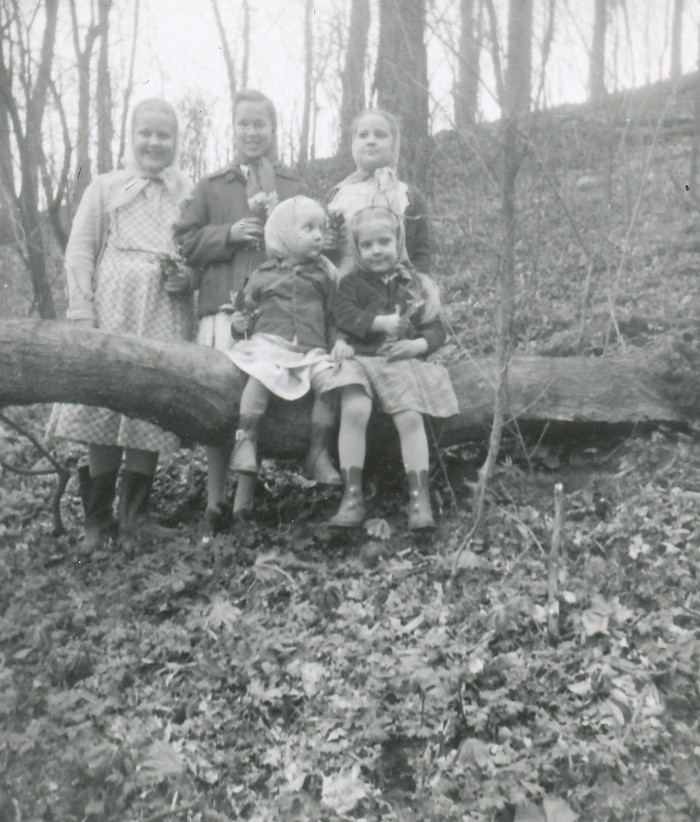
\includegraphics[width=0.9\textwidth]{reflections/5.jpg}
\caption{
Cora and Willis Stauffer
}
\end{figure}
My grandmother Cora Warfel worked with him but I know little about her family and land.
Willis died of pneumonia when my mother was 12 years old.
Cora died in 1944 leaving 6 unmarried children.
I can say that my 3 aunts who did not marry raised their younger siblings.
A memory I have of their place (along the Old Philadelphia Pike) includes a large garden.
In the fall we would go and help them dig and collect the white potatoes from the ground.

As for how land impacted relationships at church and elsewhere there are only a few things I might mention.
I believe that my father was a respected farmer in his community.
He was given responsibilities in the church and while he was in the lot for ordained leadership he was not chosen.
He served as Sunday school superintendent for a number of years.
He served on the board of New Danville Mennonite School for quite some time.
All 11 of his children attended there for 8 years.
He was glad to have sons to take over the farm when he left and now the sixth generation of Hess's seem poised to continue the farming opportunity.

\begin{figure}
\centering
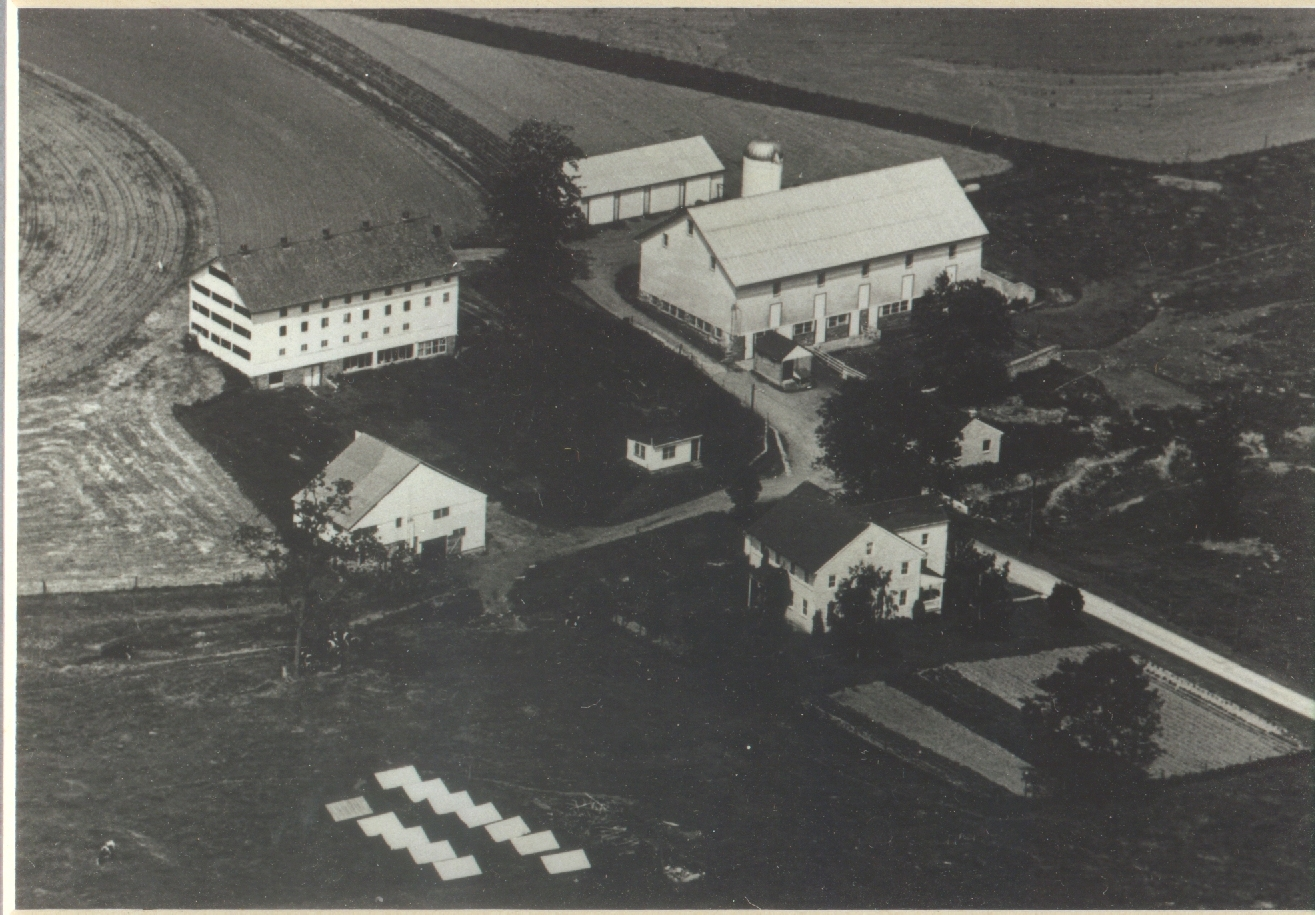
\includegraphics[width=0.9\textwidth]{reflections/7.jpg}
\caption{
Aerial view of the Hess farm on Second Lock Road
}
\end{figure}







